\documentclass[11pt, a4paper]{article}
\usepackage{graphicx}
\usepackage{amsmath}
\usepackage{listings}
\usepackage{float}


\title{Assignment No 10} % Title
\author{M Srinivas Reddy} % Author name
\date{\today} % Date for the report
\begin{document}
\maketitle
\section{Abstract}
In the previous assignments we calculated DFTs of signals and further manipulated the signals using their DFTs. One of the main uses of DFT is implementing convolution.
\section{Introduction}
In this assignment we are going to learn to calculate convolution of signals using various techniques. We are going to learn about linear and circular convolutions and also implementing convolution using DFTs.
\section{FIR Filter}
\begin{itemize}
    \item Coefficients of an FIR filter were given.
    \item  We extract these coefficients from a csv file by writing a function which opens the file and stores each row of data in a list which is later converted to an array.
    \item Using scipy.signal.freqz we plot the Magnitude and Phase plot of the filter
\end{itemize}
\begin{verbatim}
    from csv import reader
    def file(filename):
        l=[]
        with open(filename) as inp:
            for row in inp:
                l.append(float(row))
        return l
    l=file('h.csv');l=array(l)
    #Problem 2
    w,h=signal.freqz(l)
\end{verbatim}
We can see that the filter is low pass filter and has a constant group delay from the figure below.
\begin{figure}[H]
   	\centering
   	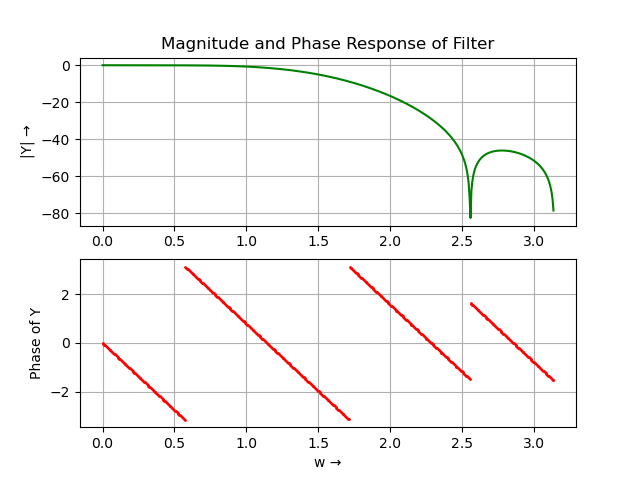
\includegraphics[scale=0.5]{Figure_1.png}
\end{figure}
\section{Convolution of Signal}
We are given a signal
\begin{equation*}
    x = cos(0.2\pi n) + cos(0.85\pi n)
\end{equation*}
We plot the signal by using the following code:
\begin{verbatim}
    N=2**10
    n=arange(1,N,1)
    x=cos(0.2*pi*n)+cos(0.85*pi*n)
    plot(n,x,color='red')
\end{verbatim}
The signal contains two frequencies: $0.2*\pi$ and $0.85*\pi$
\begin{figure}[H]
   	\centering
   	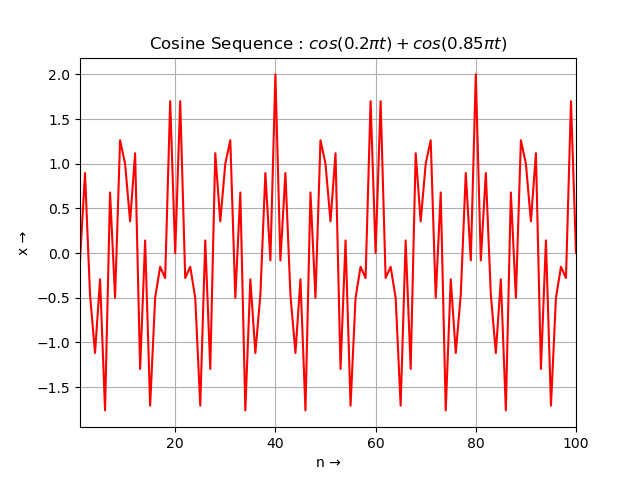
\includegraphics[scale=0.5]{Figure_2.png}
\end{figure}
\subsection{Direct Summation}
We can perform convolution of \textbf{x} and coefficients of FIR filter using direct multiplication and summation in time domain.
\begin{verbatim}
    y=signal.convolve(x,l)
    figure()
    title('Linearly Convolved Cosine Sequence')
    xlabel('n \u2192')
    ylabel('y \u2192')
    plot(range(len(n)+len(l)-1),y,color='darkviolet')
    xlim([1,100])
\end{verbatim}
The resulting signal is a sinusoid with a frequency of 0.2pi, as it is a low pass filter.
\begin{figure}[H]
   	\centering
   	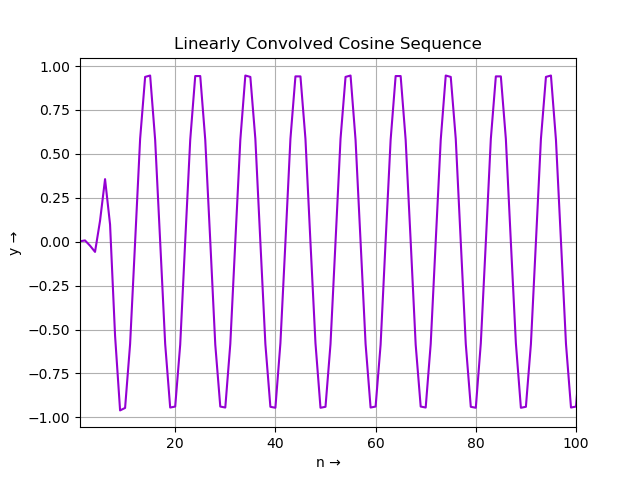
\includegraphics[scale=0.5]{Figure_3.png}
\end{figure}
\textbf{Computational Cost:}Direct Summation is most costly in terms of computation time as each multiplication and addition for an index costs a single computation.In total it costs $N^2$ computations.
\subsection{Linear Convolution using DFT}
We know that convolution in time domain is multiplication in frequency domain.So we find DFT of x and FIR filter and multiply them.
\begin{verbatim}
    x_=concatenate((x,zeros(len(l)-1)))
    l_=concatenate((l,zeros(len(x)-1)))
    y1=ifft(fft(x_)*fft(l_))
    figure()
    title('Convolvution of Cosine Sequence using DFT')
    xlabel('n \u2192')
    ylabel('y1 \u2192')
    plot(range(len(y1)),real(y1),color='hotpink')
    xlim([1,100])
\end{verbatim}
We make sure that we zero pad the signals so they are of the same length before finding the DFT and multiplying them.
\begin{figure}[H]
   	\centering
   	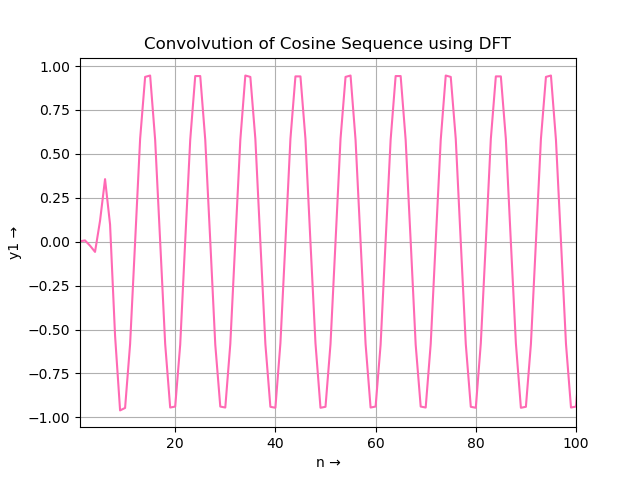
\includegraphics[scale=0.5]{Figure_4.png}
\end{figure}
\textbf{Computational Cost:}
To find DFT we need $log_{2}N$ operations.
\begin{equation}
    X[k] = \sum_{n=0}^{N-1}x[n]exp^{(-j*2\pi/N)*kn}
\end{equation}
\begin{equation}
    Y[k] = X[k]*H[k]
\end{equation}
Therefore for finding the resulting signal we require $2Nlog_{2}N+N$ operations which is less than $N^2$.
\subsection{Linear Convolution using Circular Convolution}
To perform this operation we need to implement the following steps.
\begin{itemize}
    \item We first zero pad h[n] to fit a $2^m$ window.
    \item We then divide x[n] into sections that are $2^m$ long.
    \item We then convolve sections of x[n] with h[n] and store them in an array y[n].
    \item Using a for loop we add and extend the y[n] array which has the correct values only after all the operations are done.
\end{itemize}
\begin{verbatim}
    p=len(l)
    n_=int(ceil(log2(p)))
    l_=concatenate((l,zeros(2**n_-p)))
    p=len(l_)
    n1=int(ceil(len(x)/2**n_))
    x_=concatenate((x,zeros(n1*int(2**n_)-len(x))))
    y2=zeros(len(x_)+len(l_)-1)
    for i in range(n1):
        temp=concatenate((x_[i*p:(i+1)*p],zeros(p-1)))
        y2[i*p:(i+1)*p+p-1]+=real(ifft(fft(temp)
        *fft(concatenate((l_,zeros(len(temp)-len(l_)))))))
\end{verbatim}
The output is similar to the signals obtained by using previous methods.
\begin{figure}[H]
   	\centering
   	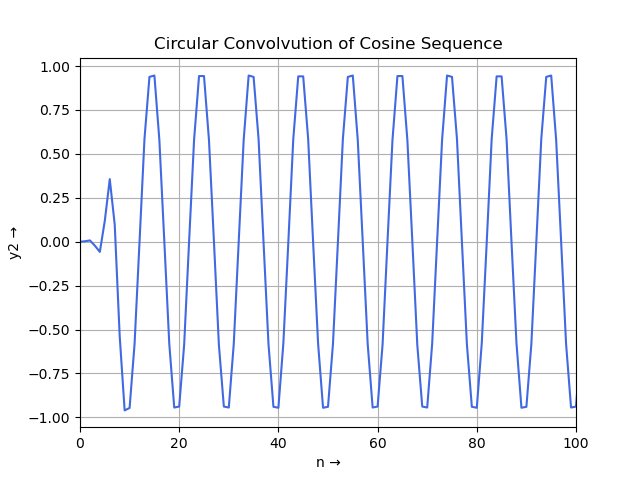
\includegraphics[scale=0.5]{Figure_5.png}
\end{figure}
\textbf{Computation Cost:}We do one N-Point DFT, N multiplications and additions and an N-point inverse DFT. Then we add the end values of y[n] (Lets say P-1). So total cost is:
\begin{equation}
    2Nlog_{2}N + N + P-1
\end{equation}
Direct linear convolution of L samples is L*P = (NP +1)P.\\
As long as $2log_(2)N + 1 <P$ the circular convolution is faster than linear convolution.
\section{Circular Correlation}
In this section, we will take an example sequence which is widely used in communications called as Zadoff-Chu sequences.\\*\\*
\textbf{Properties of Zadoff-Chu sequence:}
\begin{itemize}
    \item It is a complex sequence.
    \item It is a constant amplitude sequence.
    \item The auto correlation of a Zadoff–Chu sequence with a cyclically shifted version
of itself is zero.
    \item Correlation of Zadoff–Chu sequence with the delayed version of itself will give
a peak at that delay.
\end{itemize}
We can test the auto correlation property of Zadoff-Chu sequence by correlating with delayed version of it.(5 to the right).\\
First we need to extract the complex numbers from the csv file which is slightly different from previous method.
\begin{verbatim}
    rows=[]
    with open('x1.csv') as zadf:
        csvreader = csv.reader(zadf)
        for row in csvreader:
            rows.append(row)
    rows2=[]
    for row in rows:
        row = list(row[0])
        try:
            row[row.index('i')]='j'
            rows2.append(row)
        except ValueError:
            rows2.append(row)
            continue
    x1=[complex(''.join(line)) for line in rows2]
\end{verbatim}
We will correlate the sequences using correlate function in scipy.
\begin{verbatim}
    x2=roll(x1,5)
    zer=ifftshift(correlate(x2,x1,'full'))
    stem(arange(0,len(zer),1),
    abs(zer),'g',use_line_collection=True)
\end{verbatim}
From the below figure we can clearly see that there is a spike at 5 and zero everywhere else.
\begin{figure}[H]
   	\centering
   	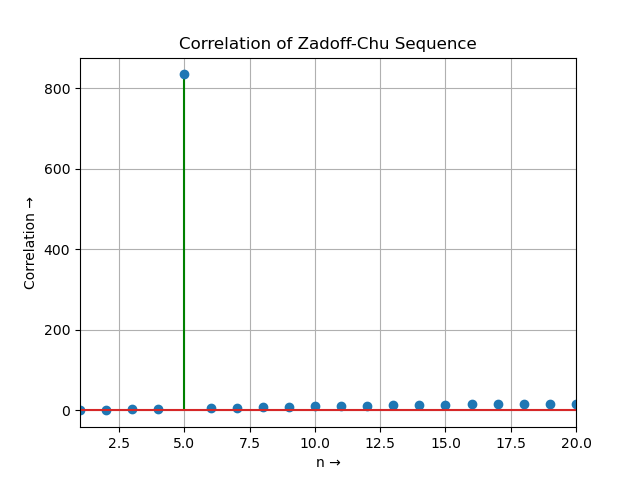
\includegraphics[scale=0.5]{Figure_6.png}
\end{figure}
\section{Conclusion}
Linear convolution algorithm implemented using a direct summation is nonoptimal and computationally expensive. A faster way to perform the convolution is to use the DFTs of the input and the filter. Circular convolution can be used for the implementation of linear convolution, with a much faster computation speed. The magnitude and phase response of a low pass filter were studied and the system’s output, for a mixed frequency signal was obtained through three different methods. For the Zadoff-Chu sequence, the auto correlation output with a cyclically shifted version of itself was found
to be non zero only at the point corresponding to the shift.
\end{document}
